\documentclass{standalone}
\usepackage{tikz}
\usetikzlibrary{}
\usepackage{bm}
\begin{document}
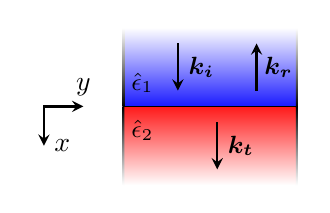
\begin{tikzpicture}
    
    % Axes
    \draw[white] (-1.4,0) -- (-1.3,0);
    \draw[thick,->, >=stealth] (-1.2,0) -- (-1.2,-0.5) node[right]{$x$};
    \draw[thick,->, >=stealth] (-1.21,0) -- (-0.7,0) node[above]{$y$};
    
    \shade[bottom color=blue!90, top color=white] (-0.2,0) -- (2,0) -- (2,1) -- (-0.2,1) -- (-0.2,0);
    \shade[bottom color=white, top color=red!90] (-0.2,0) -- (2,0) -- (2,-1) -- (-0.2,-1) -- (-0.2,0);
    
    \draw[thin] (-0.2,0) -- (2,0);
    
    \shade[bottom color=black, top color=white] (-0.2,0) -- (-0.2,1) -- (-0.18,1) -- (-0.18,0) -- (-0.2,0);
    \shade[bottom color=black, top color=white] (2,-0.01) -- (2,1) -- (2.02,1) -- (2.02,-0.01) -- (2,-0.01);
    
    \shade[bottom color=white, top color=black] (-0.2,0) -- (-0.2,-1) -- (-0.18,-1) -- (-0.18,0) -- (0,0);
    \shade[bottom color=white, top color=black] (2,0) -- (2,-1) -- (2.02,-1) -- (2.02,0) -- (2,0);
    
    \draw[thick,->, >=stealth] (0.5,0.8) -- (0.5,0.2);
    \draw[thick,->, >=stealth] (1.5,0.2) -- (1.5,0.8);
    \draw[thick,->, >=stealth] (1,-0.2) -- (1,-0.8);
    
    % Text
    \node[align=left] at (0.8,0.5) {\small $\bm{k_i}$};
    \node[align=right] at (1.78,0.5) {\small $\bm{k_r}$};
    \node[align=left] at (1.3,-0.5) {\small $\bm{k_t}$};
    
    \node[align=left] at (0.05,0.3) {\small $\hat{\epsilon}_1$};
    \node[align=left] at (0.05,-0.3) {\small $\hat{\epsilon}_2$};
    
\end{tikzpicture}
\end{document}